\documentclass[12pt]{article}			

\usepackage[utf8]{inputenc}	% az alábbi 3 sor az ékezetes betűkhöz
\usepackage[T1]{fontenc}
\usepackage{lmodern}
\usepackage{pifont}
\usepackage[english]{babel} % magyar szótagoláshoz
\usepackage{graphicx} % képek
\usepackage{pdfpages}
\usepackage{fancyhdr} % header és footer kezeléshez
\usepackage{cite}
\usepackage{enumerate} %listázáshoz
\usepackage{amsmath}
\usepackage{eqnarray}
\usepackage{gensymb} %\degree
\usepackage{float} %[H]
\usepackage{mathtools}
\usepackage{hyperref}
\hypersetup{colorlinks=false,pdfborder={0 0 0},}\usepackage[a4paper, top=1in, bottom=1in, left=1in, right=1in]{geometry} %margókhoz
\usepackage[bold]{hhtensor} % matrix, vector
\usepackage{caption}
\usepackage{enumitem}

\pagestyle{fancy}
\fancyhf{}
\fancyhead[LE,RO]{Color rampage team}
\fancyhead[RE,LO]{Deep Learning project}
\fancyfoot[RE,RO]{\thepage}
\graphicspath{{./abrak/}}  % tell LaTeX where to look for images

\usepackage{listings}
\usepackage{color}

\definecolor{dkgreen}{rgb}{0,0.6,0}
\definecolor{gray}{rgb}{0.5,0.5,0.5}
\definecolor{mauve}{rgb}{0.58,0,0.82}

\lstset{frame=tb,
	language=Python,
	aboveskip=3mm,
	belowskip=3mm,
	showstringspaces=false,
	columns=flexible,
	basicstyle={\small\ttfamily},
	numbers=none,
	numberstyle=\tiny\color{gray},
	keywordstyle=\color{blue},
	commentstyle=\color{dkgreen}\textit,
	stringstyle=\color{mauve},
	breaklines=true,
	breakatwhitespace=true,
	tabsize=3
}

\begin{document}
\begin{titlepage}
	\vspace*{100pt}
	\begin{center}
		{\Huge Deep learning \LARGE(BMEGT52AT07)}\\[3ex]
		{\Huge \bfseries Coloring grayscale images }\\[5ex] 
		{\LARGE \textit{Color Rampage team }}\\[10ex]
		{\LARGE Varjas István Péter \& Vitanov George}\\[2ex]
		{\Large \texttt{LD2J77} \hspace{4cm} \texttt{FVX4K2}}\\[2ex]
		{\Large varjas.pista@gmail.com \hspace{0.5cm} vitanovg0@gmail.com}\\[10ex]
		{\Large 2018/19. ősz}\\[10ex]
		\vspace{185pt}
	\end{center}
	
	\begin{figure}[h]
		%\includegraphics[height=50pt]{unnamed}
		\hspace{180pt}
		%\includegraphics[height=50pt]{bme_logo_nagy}\\	
		\label{fig:0}
	\end{figure}
	
\end{titlepage}
%
%\tableofcontents
%
\newpage
\section{Task description}
Our task is to colorise grayscale images. We deciced to focus on grayscale portrait pictures, because most of the old pictures taken before the popularisation of color photograpy were portraits. Our main goal is to achive accurate colorisation of the human face.
\newline\newline\noindent
To accomplish our task, we used LAB color space images. In the next section, you can read about the properties of such images, but if you are already familiar with them, just skip to the "Database" section.

\section{LAB color space}
The Lab color space consist of 3 elements:
\begin{enumerate}
	\setlength\itemsep{0.37em}
	\item \textbf{L} – Lightness ( Intensity ).
	\item \textbf{a} – color component ranging from Green to Magenta.
	\item \textbf{b} – color component ranging from Blue to Yellow.
\end{enumerate}
\vspace{4pt}
In RGB color space the color information is separated into three channels but the same three channels also encode brightness information. On the other hand, in Lab color space, the L channel is independent of color information and encodes brightness only. The other two channels encode color. \cite{lab_article}\cite{lab_wiki}
\newline\newline

\noindent This results in the following properties
\begin{itemize}
	\setlength\itemsep{0.4em}
	\item Perceptually uniform color space which approximates how we perceive color.
	\item Independent of device ( capturing or displaying ).
	\item Used extensively in Adobe Photoshop.
	\item Is related to the RGB color space by a complex transformation equation.
\end{itemize}

\begin{figure}[H]
	\centering
	\captionsetup{justification=centering}
	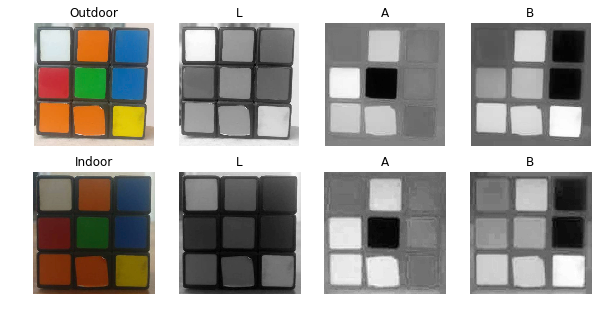
\includegraphics[height=150pt]{components-lab}
	\caption{\textbf{The Lightness ( L ), and color components \newline ( A, B ) in LAB Color space.}}	
	\label{fig:3}
\end{figure}
\newpage
\noindent Lets examine 2 images in LAB color space separated into 3 channels:
\begin{itemize}
	\item The change in illumination has mostly affected the L component.
	\item The A and B components which contain the color information did not undergo massive changes.
	\item The respective values of Green, Orange and Red ( which are the extremes of the A Component ) has not changed in the B Component and similarly the respective values of Blue and Yellow ( which are the extremes of the B Component ) has not changed in the A component.
\end{itemize}

\section{Database}
We decided on using one particular database, but besides this, we found a good collection of portrait databases:\cite{portraitdata}
\subsection{Main parameters}
Our intput database:
\begin{itemize}
	\setlength\itemsep{0.3em}
	\renewcommand\labelitemi{--}
	\item IMDB database\cite{database}, with cropped images of faces\cite{dataset}
	\item JPEG format files
	\item Variable sizes and aspect ratios
	\item Mostly small images \textasciitilde10-100 kb
	\item Containing grayscale and faulty images
\end{itemize}
\vspace{6pt}
\subsection{Faulty images}
Our database contained faulty images:
\begin{figure}[H]
	\centering
	\captionsetup{justification=centering}
	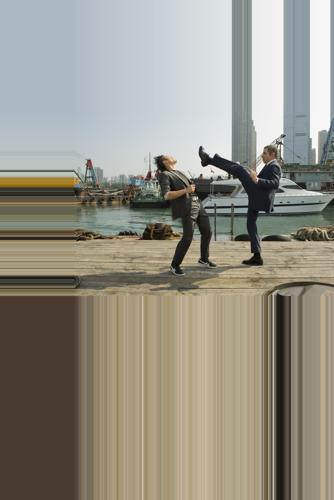
\includegraphics[height=150pt]{faulty1}
	\hspace{60pt}
	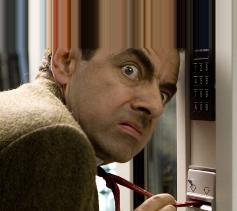
\includegraphics[height=150pt]{faulty2}
	\caption{Obviously faulty images, stripes on: (most edges; top)}	
	\label{fig:stripe_obv}
\end{figure}
\noindent It can be seen on the above figure that a faulty image contains vertical or horisontal stripes. The above two image is easily recognisible as fautly, but we found less obvius cases too:

\begin{figure}[H]
	\centering
	\captionsetup{justification=centering}
	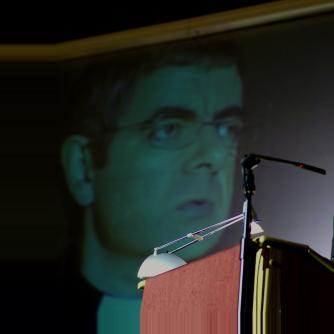
\includegraphics[height=150pt]{faulty3}
	\hspace{60pt}
	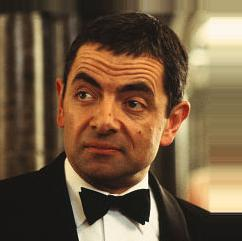
\includegraphics[height=150pt]{faulty4}
	\caption{Slightly faulty images, stripes on: (bottom; right side)}	
	\label{fig:stripe_slight}
\end{figure}
\noindent A faulty image has stripes along at least one of its edges. In one stripe (a line of pixels) all pixels have the same colour (value). This means, if we calculate the deviation of the pixel values in one stripe, we should get 0. If the image is faulty, it has at least one side, which is fully striped. This means, we can examine an image, by summing the deviation of the pixelvalues in each line of pixels on each side of an image. If on any side, the sum of the deviations results in 0, that side is striped, so the image is faulty.
\newline\newline
We decided to examine only the outer 5 pixels on each side of an image, because this proved sufficent to eliminate all faulty image. Our code for this task is:

\lstset{language=Python}
\begin{lstlisting}
def faulty(args): # Function to determine if an image is faulty
	dev = np.zeros(4)  
	val = np.zeros(4)  
	err = 5                     # we check on the first 5 pixels if stripes exist
	errp = args.shape[1]-err # and on the last 5 pixels
	for i in range(args.shape[1]):
		for j in range(3):
			val[0] = np.std(args[errp:,i,j]) # this is the i-th column pixels from 
			val[1] = np.std(args[:err,i,j])      # 123:i to 128:i and the j.th 
			val[2] = np.std(args[i,errp:,j]) # value (L,A,B)
			val[3] = np.std(args[i,:err,j])
		chopnb(val) # Activation limit because std gives small numbers (e-15) 
		dev += val   # for a list even if it contains the same elements 
# if the 0-err (0-5) and the errp-lastpixel (123-128) pixelrange does not 
# contain stripes then:
	if (dev[0] != 0 and dev[1] != 0 and dev[2] != 0 and dev[3] != 0):
		return 0
	else:
	return 1
\end{lstlisting}

\subsection{Grayscale images}
\begin{figure}[H]
	\centering
	\captionsetup{justification=centering}
	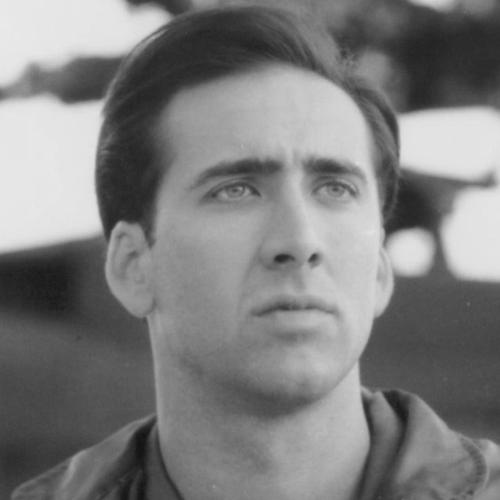
\includegraphics[height=140pt]{graysc1}
	\hspace{60pt}
	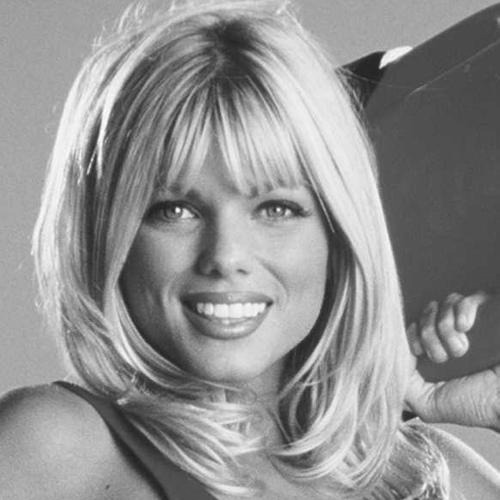
\includegraphics[height=140pt]{graysc2}
	\caption{Grayscale images}	
	\label{fig:grayscale_eg}
\end{figure}
Our database contained grayscale images too. We examined the images in LAB color space, because unlike in RGB, in LAB they can be easily recognisible as greyscale. Lets examine a 5x5 pixel grayscale image of a flamingo:

\begin{figure}[H]
	\centering
	\captionsetup{justification=centering}
	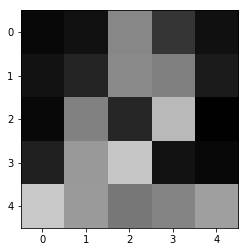
\includegraphics[height=150pt]{flamingo}
	\caption{Grayscale flamingo 5x5 pix}	
	\label{fig:grayscale_flam}
\end{figure}

\begin{figure}[H]
\centering
\begin{equation*}
\begin{pmatrix}
8 & 17 & 135 & 53 & 16 \\
18 & 35 & 138 & 128 & 27 \\
8 & 129 & 38 & 185 & 1 \\
32 & 153 & 198 & 18 & 8 \\
200 & 154 & 119 & 132 & 159 \\
\end{pmatrix}
\begin{pmatrix}
8 & 17 & 135 & 53 & 16 \\
18 & 35 & 138 & 128 & 27 \\
8 & 129 & 38 & 185 & 1 \\
32 & 153 & 198 & 18 & 8 \\
200 & 154 & 119 & 132 & 159 \\
\end{pmatrix}
\begin{pmatrix}
8 & 17 & 135 & 53 & 16 \\
18 & 35 & 138 & 128 & 27 \\
8 & 129 & 38 & 185 & 1 \\
32 & 153 & 198 & 18 & 8 \\
200 & 154 & 119 & 132 & 159 \\
\end{pmatrix}
\end{equation*}
\caption{R G B channels respectively} %a caption a label előtt legyen
\label{fig:kep4}
\end{figure}

\begin{figure}[H]
	\centering
	\begin{equation*}
	\begin{pmatrix}
	2 & 5 & 56 & 22 & 4 \\
	5 & 13 & 57 & 53 & 9 \\
	2 & 53 & 15 & 75 & 0 \\
	12 & 63 & 79 & 5 & 2 \\
	80 & 63 & 50 & 55 & 65 \\
	\end{pmatrix}
	\begin{pmatrix}
	0 & 0 & 0 & 0 & 0 \\
	0 & 0 & 0 & 0 & 0 \\
	0 & 0 & 0 & 0 & 0 \\
	0 & 0 & 0 & 0 & 0 \\
	0 & 0 & 0 & 0 & 0 \\
	\end{pmatrix}
	\begin{pmatrix}
	0 & 0 & 0 & 0 & 0 \\
	0 & 0 & 0 & 0 & 0 \\
	0 & 0 & 0 & 0 & 0 \\
	0 & 0 & 0 & 0 & 0 \\
	0 & 0 & 0 & 0 & 0 \\
	\end{pmatrix}
	\end{equation*}
	\caption{L A B channels respectively} %a caption a label előtt legyen
	\label{fig:kep5}
\end{figure}

\noindent On the above figures, we can see, that working in the LAB color space gives us the opportunity, to identify a grayscale image by its A and B matrices. An image is therefore grayscale if we sum the absolute values of its pixels in channel A and B respectively, and get zero as a cumulative sum.
\newline 
\newline First we define a function for iterating and abs[] function on arrays. Then we can sum up the individual array elements with numpy.sum()

\begin{lstlisting}
def abbs(expr): #defining Abs function for arrays
	return [abs(i) for i in expr]
	
#check if image is grayscale, if not add it to image array
if (np.sum(abbs(img[:,:,1]))+np.sum(abbs(img[:,:,2]))!= 0): 
	img_array.append(img)
\end{lstlisting}

\section{Data processing}

\subsection{Crop function}
As mentioned before our database contained images in various aspect ratios. When using PIL.Image.resize() function, we encountered a problem, that this funtcion did not keep the original aspect ratio of the pictures, but rather compressed/elongated them. To overcome this problem, we created a crop funtion. The output of our function is a 1:1 aspect ratio image, with the excess sides or excess stripes on the top and bottom simmetrically removed.

\begin{figure}[H]
	\centering
	\captionsetup{justification=centering}
	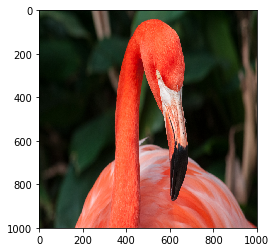
\includegraphics[height=140pt]{flam_sm}
	\hspace{1cm}
	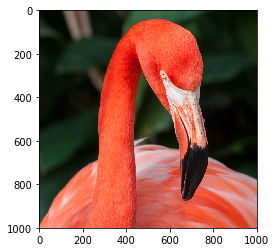
\includegraphics[height=140pt]{flam_crp}
	\caption{Resized without crop, Resized with crop}	
	\label{fig:flam_diff}
\end{figure}

\noindent Our function to crop a picture to a square shape, with cropping the edges, and giving the max middle square back:
\begin{lstlisting}
def cropmid(img): 
	if(img.size[0]!= img.size[1]): # check if img needs cropping first
		xfrom = int((img.size[0]-min(img.size))/2) # we crop from here
		xto = xfrom+min(img.size)                       # til here
		yfrom = int((img.size[1]-min(img.size))/2)
		yto = yfrom+min(img.size)

		return img.crop((xfrom,yfrom,xto,yto))
	else:
		return img
\end{lstlisting}

\subsection{File format}
Our task does not require complex data structures, so after some experiments we decided to use .csv file format to store our data. A .csv file generally stores 2d arrays, which is perfect for storing our fix-sized images. It was also an important criteria, that the file should be easily appendable and could be partially read if nessesarry. A .csv is also fast to generate and easy to use. The figure below shows how we store pixel values in .csv format.
\begin{figure}[H]
	\centering
	\captionsetup{justification=centering}
	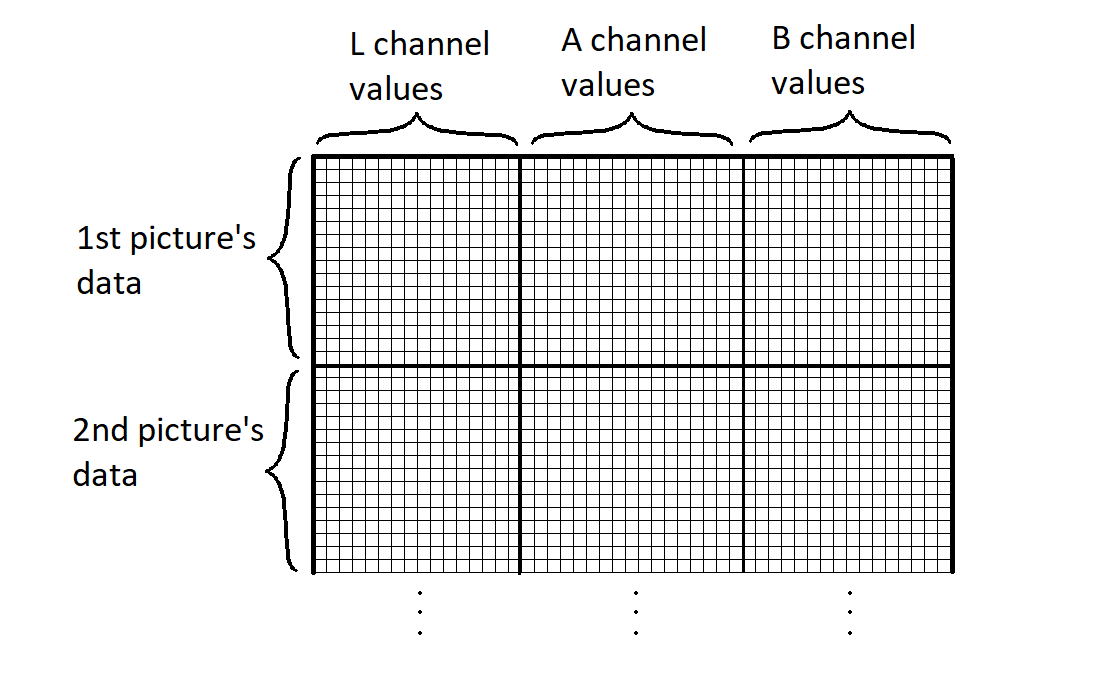
\includegraphics[height=250pt]{data_storing}
	\caption{Data storing}	
	\label{fig:d_s}
\end{figure}
\subsection{Backup}
Our code works by sorting a predetermined number of good images (\textasciitilde 16 000), then saveing their LAB pixel values:
\begin{lstlisting}
with open('D:/EVTNG/Dataset/csv_v3/labpics.csv', 'w+',newline='') as out:
writer = csv.writer(out, delimiter = ',')
for ind in range(len(pix)):
writer.writerows(np.round(np.concatenate((pix[ind][:,:,0], \
pix[ind][:,:,1], pix[ind][:,:,2]), axis = 1)).astype(np.int))
\end{lstlisting}

\noindent We can read the values back with pandas relatively fast:
\begin{lstlisting}
import pandas as pd
df = pd.read_csv('D:/EVTNG/Dataset/csv_v3/labpics.csv', header=None, dtype = np.float32)
data = df.as_matrix()
\end{lstlisting}
\subsection{Creating learning data}
We used normalization on the input as well as on the output, because the range of our data (each channel's value range) is predetermined. By choosing this method we can easily expand our learning data if nessesarry. (otherwise the recalculation of the deviation and average for the whole dataset would be nessessarry)

\subsection{Performance measurements}
We measured the performance of different data processing and saving techniques on 10000 images. Data saveed by the python function pickle, will be referred to as .p file format.
\begin{figure}[H]
	\centering
	\captionsetup{justification=centering}
	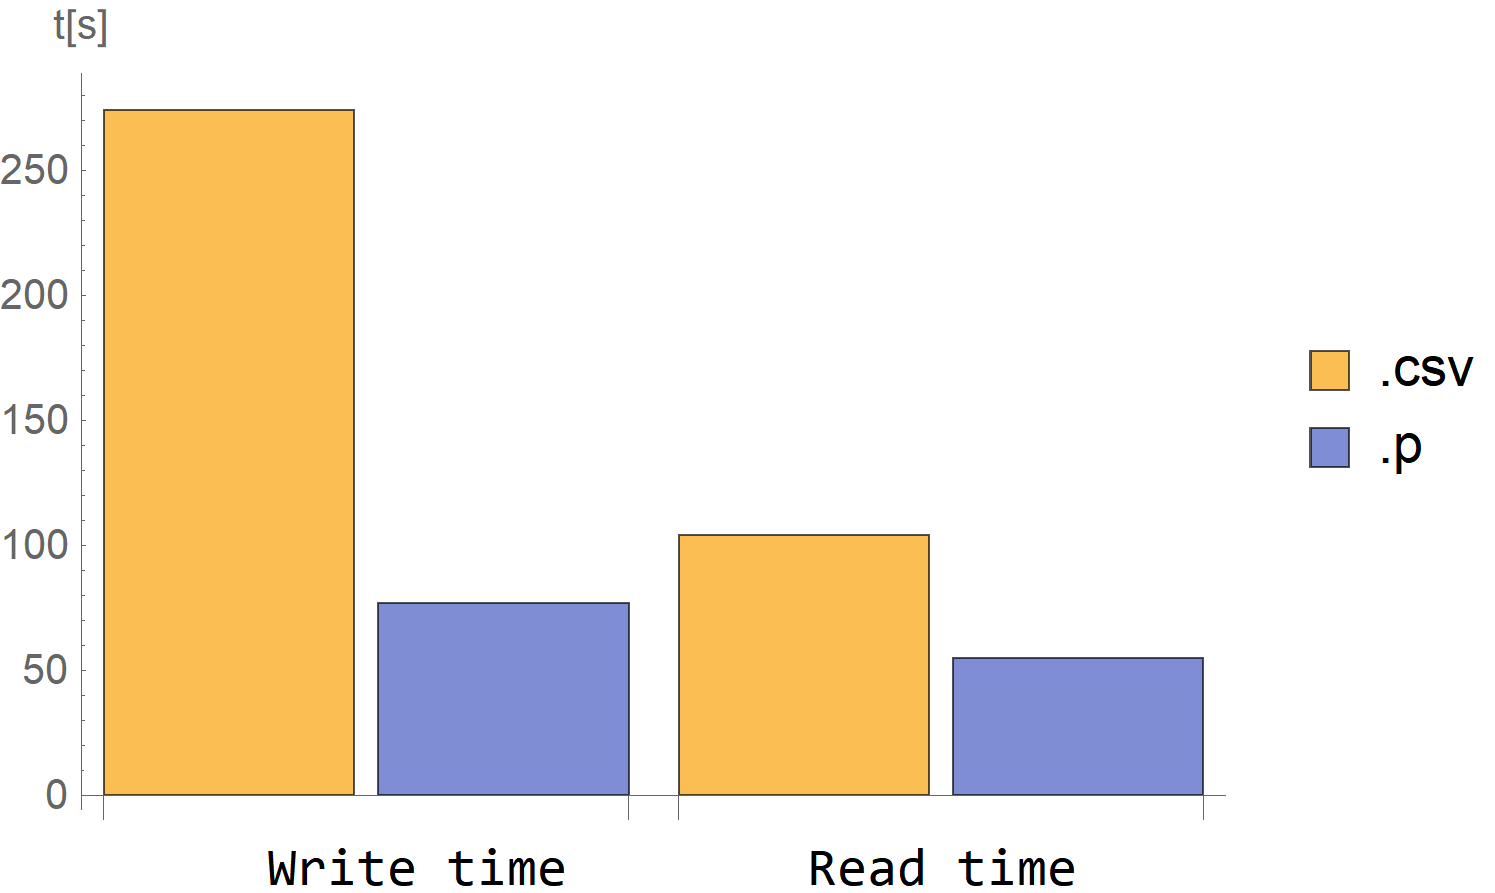
\includegraphics[height=150pt]{plot_2}
	\caption{Time to process 10 000 images, using .csv and .p file types}	
	\label{fig:data_proc_time}
\end{figure}
\begin{figure}[H]
	\centering
	\captionsetup{justification=centering}
	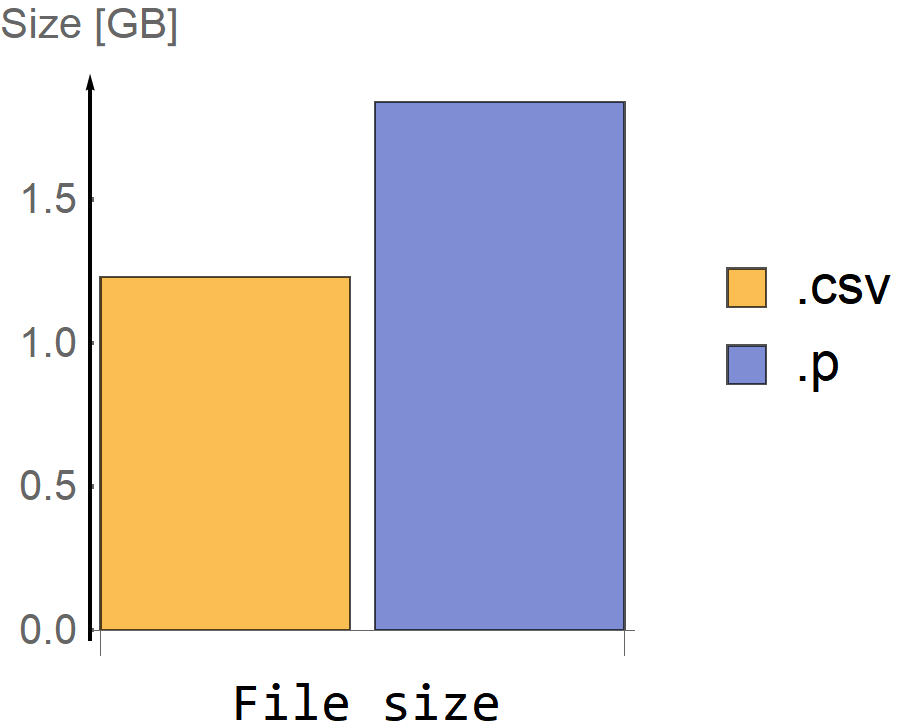
\includegraphics[height=150pt]{plot_1}
	\caption{Data size: 10 000 images, using .csv and .p file types}	
	\label{fig:data_proc_size}
\end{figure}
\noindent The above numbers are measured means of data processing times and data sizes. We usually did each measurement with the same data 5 times. Although we achieved far better times with pickleing the data (.p) we decided to use (.csv) fileformat, because of the reduced filesize and the useability of a .csv file. (A .csv file is generally interpretable for any program, while pickeling our data gives us a file only interpretable by python.)\newline\newline\newline
\begin{Large}
\textbf{Collection of image colorization Deep Learning solutions:}
\end{Large}
\begin{itemize}
	\setlength\itemsep{0em}
	\renewcommand\labelitemi{--}
	\item \href{https://arxiv.org/abs/1603.08511}{Colorful Image Colorization}
	\item \href{https://arxiv.org/abs/1605.00075}{Deep Colorization}
	\item \href{https://arxiv.org/abs/1611.07004}{Image-to-Image Translation with Conditional Adversarial Networks}
	\item \href{https://arxiv.org/abs/1803.05400}{Image Colorization with Generative Adversarial Networks}
	\item \href{https://arxiv.org/abs/1604.07904}{Image Colorization Using a Deep Convolutional Neural Network}
	\item \href{https://arxiv.org/abs/1704.04610}{A learning-based approach for automatic image and video colorization}
	\item \href{https://www.learnopencv.com/convolutional-neural-network-based-image-colorization-using-opencv/}{Convolutional Neural Network based Image Colorization using OpenCV}
\end{itemize}
\begin{thebibliography}{sort}
	\bibitem{lab_article}\url{https://www.learnopencv.com/color-spaces-in-opencv-cpp-python/}
	\bibitem{lab_wiki}\url{https://en.wikipedia.org/wiki/CIELAB_color_space}
	\bibitem{database}\url{https://data.vision.ee.ethz.ch/cvl/rrothe/imdb-wiki/}
	\bibitem{dataset}\url{https://data.vision.ee.ethz.ch/cvl/rrothe/imdb-wiki/static/imdb_crop.tar}
	\bibitem{portraitdata}\url{http://www.face-rec.org/databases/}
	
\end{thebibliography}
\end{document}